\subsection{Resultados}
\label{sec:results_AT}
%\subsubsection{Verificación del modelo AT}

\begin{figure}[ht!]
\begin{center}
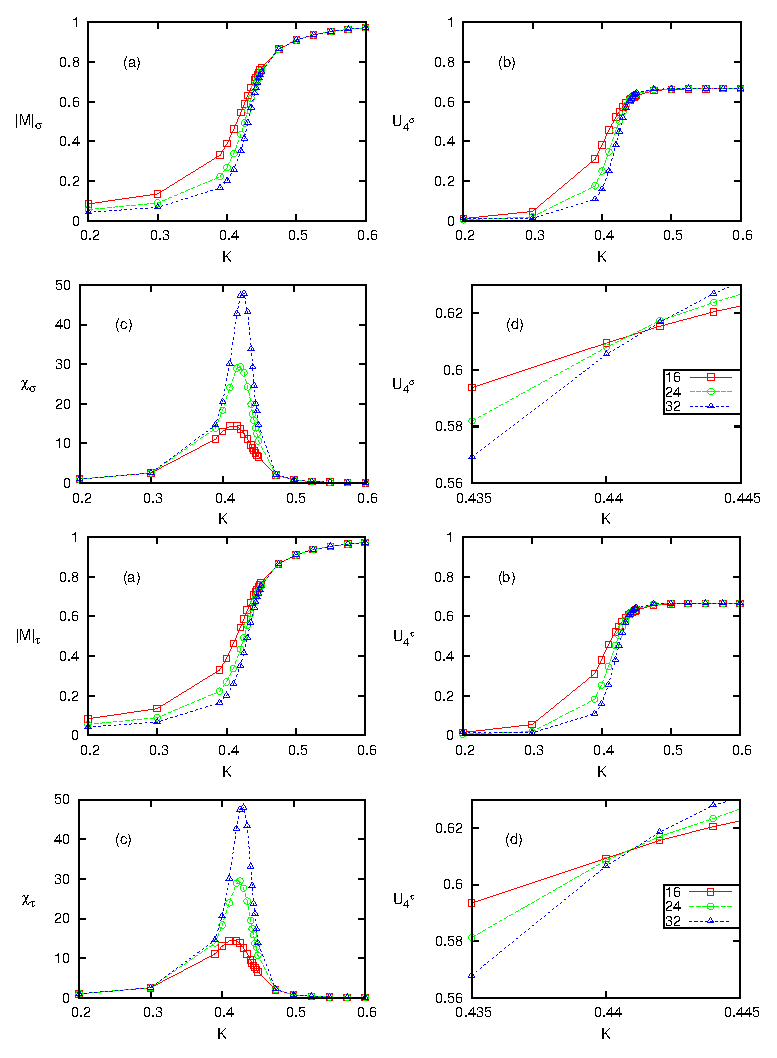
\includegraphics[scale=0.8]{graf/phases/multi_ising_sigma_tau_inkscape.eps}
\end{center}
\caption{En el caso $K_{4}=0$ el comportamiento de los spines $\sigma$ y los $\tau$ es el del modelo de Ising en una red cuadrada.
 (a): en las medidas de la magnetización del sistema ($|M_{\sigma}|=\mean{\sigma}$, $|M_{\tau}|=\mean{\tau}$) puede observarse la transici\'on de fase de segundo orden en $K_{c}^{Ising}$,
 (b): la susceptibilidad magn\'etica presenta un pico abrupto en $K_{c}^{Ising}$ que se vuelve m\'as pronunciado a medida que
 aumenta el tamaño del sistema, deber\'ia transformarse en una divergencia para $L\rightarrow \infty$.(c): A partir
 del cumulante de cuarto orden es posible determinar el punto cr\'itico para un sistema finito, (d): La ubicaci\'on del
 punto cr\'itico se obtiene de la intersecci\'on entre los cumulantes para diferentes valores de $L$.}
\label{fig:multi_ising_sigma_tau}
\end{figure}

Nuestro objetivo en esta sección es comprobar la fidelidad del algoritmo utilizado en las simulaciones con el modelo AT. Para ello estudiamos
 el comportamiento del sistema en diferentes situaciones en las que los resultados son conocidos, ya sea analíticamente o a partir de otros estudios numéricos.\\
Hemos tenido en cuenta primero la situación más sencilla, en la que el acoplamiento entre spines $\sigma$ y $\tau$, $K_{4}$, es nulo y el sistema puede separarse
 en dos modelos de Ising bidimensionales independientes. Luego abordamos el estudio del comportamiento del sistema en las diferentes fases descriptas en
 la sección \ref{sec:AT_model} y la determinación de las líneas críticas que se observan en el diagrama de la Fig. \ref{fig:AT_ph_diag_Baxter}. Por último antes de considerar
 el sistema con defectos, estudiamos el comportamiento no universal del exponente crítico de la magnetización en el modelo AT sobre la línea E-F del diagrama de fases.\\

%\begin{figure}[ht!]
%\begin{center}
%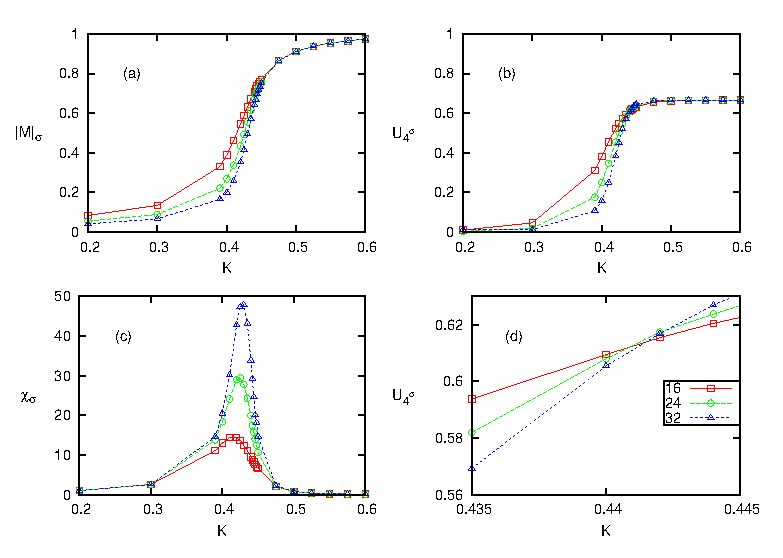
\includegraphics[scale=0.8]{graf/phases/multi_ising_sigma.eps}
%\end{center}
%\caption{En el caso $K_{4}=0$ el comportamiento de los spines $\sigma$ es el del modelo de Ising en una red cuadrada.
 %(a): en las medidas de la magnetización del sistema ($|M|=\mean{\sigma}$) puede observarse la transici\'on de fase de segundo orden en $K_{c}^{Ising}$,
 %(b): la susceptibilidad magn\'etica presenta un pico abrupto en $K_{c}^{Ising}$ que se vuelve m\'as pronunciado a medida que
 %aumenta el tamaño del sistema, deber\'ia transformarse en una divergencia para $L\rightarrow \infty$.(c): A partir
 %del cumulante de cuarto orden es posible determinar el punto cr\'itico para un sistema finito, (d): La ubicaci\'on del
 %punto cr\'itico se obtiene de la intersecci\'on entre los cumulantes para diferentes valores de $L$.}
%\label{fig:multi_ising_sigma}
%\end{figure}

Los datos analizados en esta sección surgen de medidas realizadas para los parámetros de orden $\mean{\alpha}$, $\mean{\alpha}_{AF}$,
 $\mean{\sigma\tau}$ y $\mean{\sigma\tau}_{AF}$ ($\alpha=\sigma, \tau$), definidos en las ecuaciones \ref{eq:op_Ms}, \ref{eq:op_stagMs}, \ref{eq:op_Mst} y
 \ref{eq:op_stagMst}, y sus momentos de orden 2 y 4, a partir de los que se pueden obtener el cumulante de cuarto orden y la
 susceptibilidad (ecs. \ref{eq:cumul4} y \ref{eq:suscept}) que permiten
 caracterizar la transición de fase y determinar el punto crítico.
Dado que nuestro objetivo en esta sección es reproducir las propiedades del modelo AT sin defectos, hemos optado por considerar sistemas de tamaños relativamente
 pequeños, $L=16,24,32$, a fines de reducir el tiempo de procesamiento en cada caso.
Para estos tamaños se realizaron corridas de hasta $3\times 10^{5}$ TMC, luego de un período de equilibrio de $3\times 10^{5}$ TMC, para los tamaños más grandes,
 y realizando promedios sobre 50 muestras independientes.\\

%\begin{figure}[ht!]
%\begin{center}
%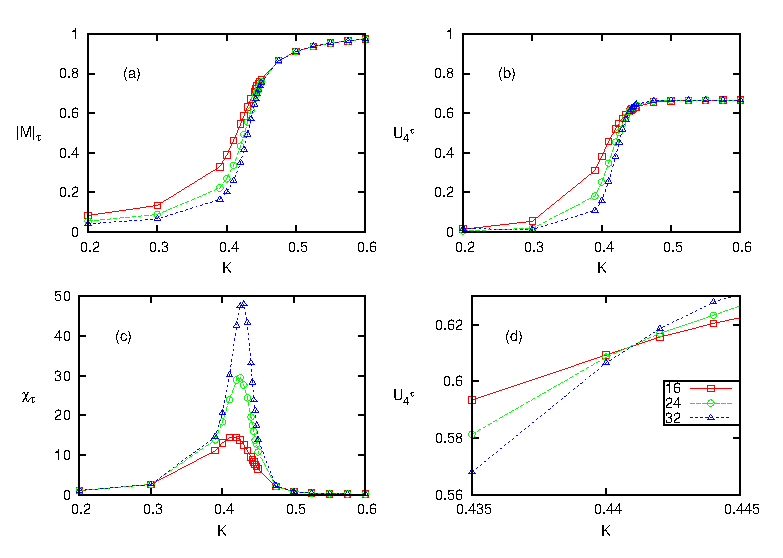
\includegraphics[scale=0.8]{graf/phases/multi_ising_tau.eps}
%\end{center}
%\caption{Esta figura es similar a la figura \ref{fig:multi_ising_sigma}, pero se representan la magnetización ($|M|=\mean{\tau}$), susceptibilidad y cumulante de cuarto orden en función de $K$
 %para los spines $\tau$ en el caso $K_{4}=0$.}
%\label{fig:multi_ising_tau}
%\end{figure}

\subsubsection{Sistema desacoplado ($K_{4}=0$)}

Consideremos en primer lugar el caso en el cual $K_{4}=0$ que corresponde a dos modelos de Ising desacoplados, para los cuales
 se espera obtener una transición de fase de segundo orden para el valor $K = K_{c}^{Ising}$ determinado por la ec. (\ref{eq:isingcrit}).
 Para analizar esta transición hemos calculado la magnetización, la susceptibilidad magnética y el cumulante de cuarto orden
 como funciones de $K$ y para diferentes valores de $L$.\\
En la Fig. \ref{fig:multi_ising_sigma_tau} puede observarse el comportamiento de (a) los parámetros de orden $\abs{M_{\sigma,\tau}}$, (b) el cumulante de cuarto orden $U_{4}$ y
 (c) la susceptibilidad magnética asociada, característicos
 de una transición de fase de este tipo. A medida que aumenta el tamaño del sistema la transición en (a) se vuelve mas abrupta y el pico de la susceptibilidad en (c) tiende
 a una divergencia. Se observa además que el comportamiento es similar para los spines $\sigma$ y los $\tau$, ya que se trata, en este caso, de dos modelos de Ising independientes.\\
 
Hemos determinado el valor crítico de la constante de acoplamiento $K_{c}^{Ising}$ localizando las intersecciones de las gráficas de $U_{4}$
 para los spines $\sigma$ y $\tau$ para diferentes tamaños del sistema, $L=16,24,32$. Éstas pueden observarse en los gráficos $(d)$ en la figura \ref{fig:multi_ising_sigma_tau}.
% y \ref{fig:multi_ising_tau}.
 Los resultados obtenidos para los spines $\sigma$ y los $\tau$ están en buen acuerdo con el valor teórico de $K_{c}^{Ising}$ (ec. \ref{eq:isingcrit}):
 $K_{c}^{\sigma}=K_{c}^{\tau}=0.441(1)$.\\


\begin{figure}[h!]
	\begin{center}
		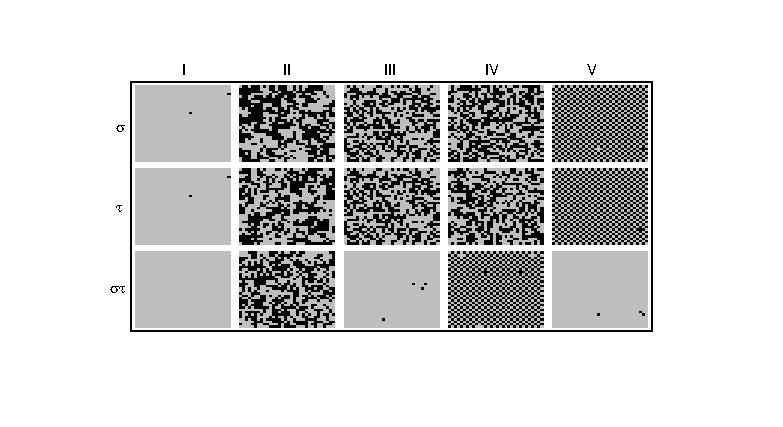
\includegraphics[scale=1]{graf/phases/multi_snaps32_horiz.eps}
	\end{center}
	\caption{Snapshots del sistema en las diferentes fases. Cada columna corresponde a una región diferente del diagrama de fases.
	En la fila superior se representan los spines $\sigma$, en la central los $\tau$ y en la inferior el producto $\sigma\tau$.
	Estos gráficos se han realizado para un sistema de tamaño $32\times 32$. Para la primera columna se ha tomado $K=0.5$ y $K_{4}=0.5$,
	es decir un estado del sistema correspondiente a la región I del diagramade fases. La segunda columna corresponde a la región II y se obtuvo con $K=0.2$ y $K_{4}=0$.
	La tercera columna se obtiene para $K=0.1$ y $K_{4}=0.75$ y pertenece la fase III. La cuarta columna }
	\label{fig:snaps_multi}
\end{figure} 

\subsubsection{Diagrama de fases para el caso acoplado $K_{4}\neq 0$}

Una vez analizado el caso desacoplado, pasamos a considerar un valor de $K_{4}$ no nulo, verificando las diferentes fases que presenta el modelo AT.
La figura \ref{fig:snaps_multi} muestra instantáneas del sistema en cada fase, imágenes que representan la red bidimensional en las que se utilizan diferentes tonalidades
 para indicar el estado de spin en que se encuentra cada sitio. Considerando solo dos tonalidades (claro y oscuro) el estado del modelo AT en un instante particular
 puede representarse por dos redes (spines $\sigma$ y $\tau$). En esta representación gráfica se hacen claras las diferentes fases asociadas a los valores de $K$ y $K_{4}$
 que se muestran en la Fig. \ref{fig:AT_ph_diag_Baxter}.
Cada columna corresponde a una de las regiones en el diagrama de fases, mientras que las filas, de arriba hacia abajo, corresponden a los estados de los spines
 $\sigma$, $\tau$ y del producto $\sigma\tau$. Estas medidas fueron realizadas para una red cuadrada de $32\times 32$.\\

En la primer columna se muestra la configuración para $K=0.5$ y $K_{4}=0.5$, que corresponde a la región I del diagrama de fases de
 la Fig. \ref{fig:AT_ph_diag_Baxter}, el sistema se encuentra completamente ordenado, todos los spines, tanto $\sigma$ como $\tau$, están en el mismo estado y
 por lo tanto también su producto.
En la columna 2 se presenta el caso $K=0.2$, $K_{4}=0$, en el que los spines $\sigma$ y los $\tau$ se encuentran desordenados de manera independiente,
 y por ello $\sigma\tau$ presenta también un estado sin orden alguno. Esto corresponde a la región II en la Fig. \ref{fig:AT_ph_diag_Baxter}.
En la columna 3 se observa como los spines $\sigma$ y $\tau$ pueden estar desordenados, mientras que su producto presenta un estado ordenado. Esta
 situación, correspondiente a la región III del diagrama de fases (Fig. \ref{fig:AT_ph_diag_Baxter}), es observada para un valor pequeño de las
 interacciones $\sigma-\sigma$ y $\tau-\tau$, $K=0.1$, y un acoplamiento relativamente fuerte para la interacción $\sigma-\tau$, $K_{4}=0.75$.
En cambio si el valor de $K_{4}$ es negativo, los spines $\sigma$ se acoplan a los $\tau$ de manera anti-ferromagnética, lo que puede verse en
 la columna 4 de la figura \ref{fig:snaps_multi} donde se ha elegido $K_{4}=-0.75$, en correspondencia con la región IV de la figura \ref{fig:AT_ph_diag_Baxter}.
Por último, en la columna 5, se ha considerado el caso en que $K$ es negativo, $K=-0.75$ y $K_{4}=0.1$, produciéndose un orden alternado para los $\sigma$ y los $\tau$,
 mientras que el producto $\sigma\tau$ permanece en un estado de orden ferromagnético. Este caso es representativo de la región V del diagrama de fases (Fig. \ref{fig:AT_ph_diag_Baxter}).\\

\begin{figure}[h!]
	\begin{center}
		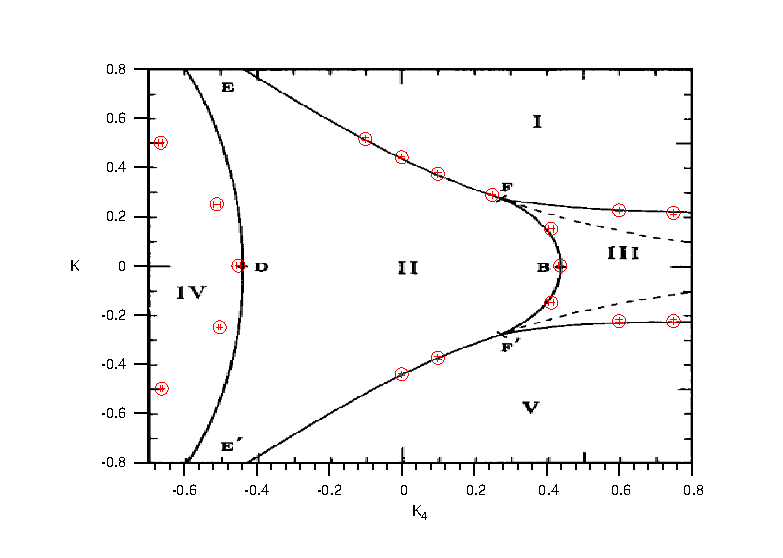
\includegraphics[scale=1]{graf/phases/new_phase_diag_back.eps}
	\end{center}
	\caption{Se presentan los puntos obtenidos en este trabajo para las transiciones de fase del modelo AT sobre el diagrama de fases publicado por Baxter\cite{baxter_book}.
	En el caso de la transici\'on II$\rightarrow$IV, la curva es solo representativa, no se ha determiando su expresi\'on anal\'itica.}
	\label{fig:phase_diag_back}
\end{figure}

\begin{figure}[h!]
	\begin{center}
		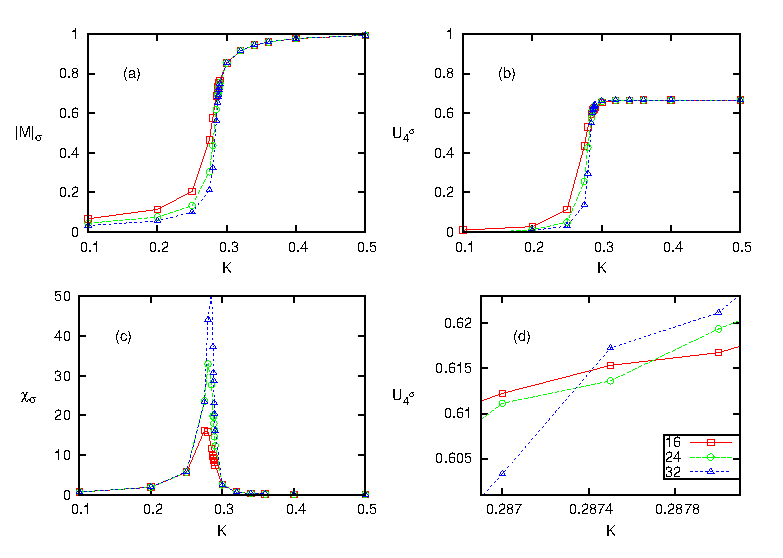
\includegraphics[scale=0.8]{graf/phases/multi_AT_I_II_c.eps}
	\end{center}
	\caption{En el caso $K_{4}=0.25$ la transición entre las fases I y II, localizada sobre la curva E-F, es similar a la que ocurre en el modelo de Ising.
	El valor crítico de $K$ es menor a $K_{c}^{Ising}$.(a): magnetización ($|M|=\mean{\sigma}$), puede observarse la transici\'on de fase de segundo orden en $K\simeq 0.287(1)$,
	(b): la susceptibilidad magn\'etica presenta un pico abrupto en $K_{c}^{Ising}$ que se vuelve m\'as pronunciado a medida que
	aumenta el tamaño del sistema, deber\'ia transformarse en una divergencia para $L\rightarrow \infty$.(c): A partir
	del cumulante de cuarto orden es posible determinar el punto cr\'itico para un sistema finito, (d): La ubicaci\'on del
	punto cr\'itico se obtiene de la intersecci\'on entre los cumulantes para diferentes valores de $L$.}
	\label{fig:multi_AT_I_II_c}
\end{figure}

\begin{figure}[h!]
	\begin{center}
		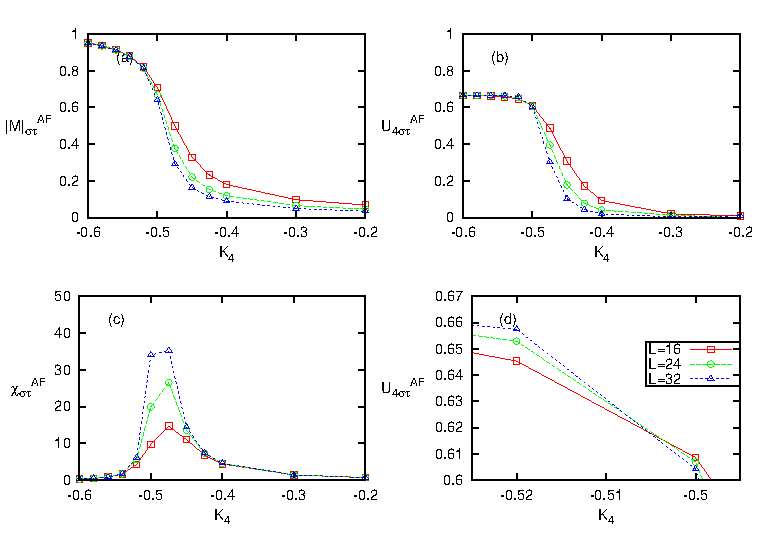
\includegraphics[scale=0.8]{graf/phases/new_multi_AT_II_IV_b.eps}
	\end{center}
	\caption{La transición entre las fases II y IV, localizada sobre la línea E-E'
	puede estudiarse mediante el parámetro de orden $\mean{\sigma\tau}_{AF}$, utilizando un valor fijo de $K=0.377$.
	El comportamiento de las magnitudes $\abs{M}_{\sigma\tau}^{AF}$, $\chi_{\sigma\tau}^{AF}$ y $U_{4\sigma\tau}^{AF}$
	corresponde al de una transici\'on de fase de segundo orden.}
	%\caption{La transición entre las fases II y III, localizada sobre la línea F-F' puede estudiarse mediante el parámetro de orden $\mean{\sigma\tau}_{AF}$.
	%El punto B se encuentra en $K=0$, $K_{4}=K_{c}^{Ising}$.(a): magnetización ($|M|=\mean{\sigma}$), puede observarse la transici\'on de fase de segundo orden en $K\simeq 0.287(1)$,
	%(b): la susceptibilidad magn\'etica presenta un pico abrupto en $K_{c}^{Ising}$ que se vuelve m\'as pronunciado a medida que
	%aumenta el tamaño del sistema, deber\'ia transformarse en una divergencia para $L\rightarrow \infty$.(c): A partir
	%del cumulante de cuarto orden es posible determinar el punto cr\'itico para un sistema finito, (d): La ubicaci\'on del
	%punto cr\'itico se obtiene de la intersecci\'on entre los cumulantes para diferentes valores de $L$.}
	\label{fig:multi_AT_II_IV_b}
\end{figure}

Mediante el mismo procedimiento que el utilizado en la transición de fase para $K_{4}=0$ % método del determinante de cuarto orden
 hemos determinado varios puntos ($K$, $K_{4}$) correspondientes a las curvas cr\'iticas del diagrama
 de la Fig. \ref{fig:AT_ph_diag_Baxter}. En la Fig. \ref{fig:phase_diag_back} se resumen
 dichos resultados numéricos superpuestos al diagrama de fases ya conocido, con el que se obtiene un excelente acuerdo,
 excepto en el caso de la curva E-D-E', en el que existe cierta diferencia. Este caso se discutirá más adelante.
%Las curvas cr\'iticas en el diagrama ($K$, $K_{4}$) para las transiciones entre las
 %fases enumeradas anteriormente han sido determinados de la misma forma que en
 %la transición para $K_{4}=0$, utilizando el método del cumulante de cuarto orden.
%Los resultados hallados para todas las transiciones de fase estudiadas concuerdan con el diagrama de fases de la Fig. \ref{fig:AT_ph_diag_Baxter},
 %y pueden verse superpuestos a este en la Fig. \ref{fig:phase_diag_back}, los c\'irculos rojos corresponden a los resultados n\'umericos obtenidos
 %en este trabajo.
Las figuras \ref{fig:multi_AT_I_II_c} y \ref{fig:multi_AT_II_IV_b} muestran el comportamiento
 de las magnitudes $\abs{M}$, $\chi$ y $U_{4}$ en las cercanías de los puntos críticos.
 La figura \ref{fig:multi_AT_I_II_c} corresponde al caso de
 la transición entre las fases I y II para un valor de $K_{4}$ diferente de $0$ donde se utiliz\'o
 $M_{\sigma}=\mean{\sigma}$ como par\'ametro de orden. Las curvas muestran el mismo comportamiento que en el caso
 $K_{4}=0$, pero puede verse que el valor crítico obtenido para $K$ es diferente.
 La figura \ref{fig:multi_AT_II_IV_b}
  corresponde a la transici\'on entre las fases II y IV, caraterizada por el parámetro de orden $\abs{M_{\sigma\tau}^{AF}}=\mean{\sigma\tau}_{AF}$,
  en los gr\'aficos (a-d) puede verse que el
  comportamiento del par\'ametro de orden $\mean{\sigma\tau}_{AF}$, la susceptibilidad $\chi_{\sigma\tau}^{AF}$
  y el cumulante de cuarto orden es el correspondiente a una transici\'on de fase de segundo orden.\\
 
\begin{figure}[h!]
	\begin{center}
		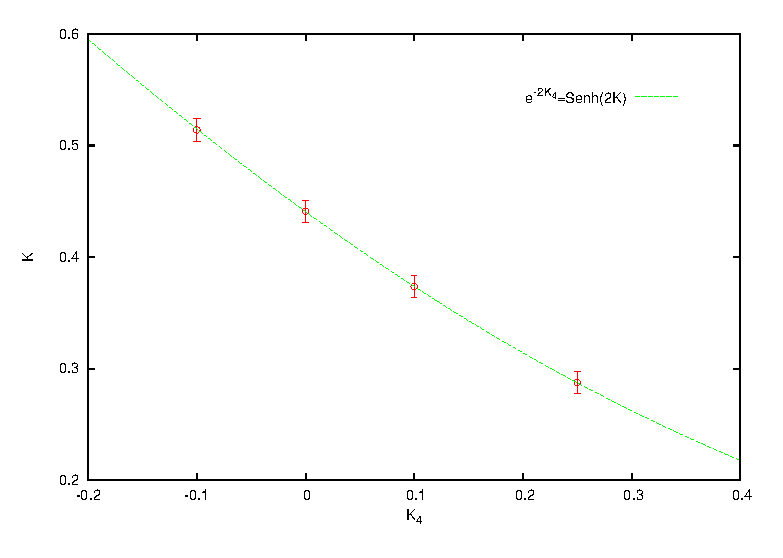
\includegraphics[scale=0.85]{graf/phases/phases_EF.eps}
	\end{center}
	\caption{Transiciones de fase sobre la línea E-F, definida por (\ref{eq:lincrit}), para diferentes valores de $K_{4}=-0.1, 0, 0.1, 0.25$. La curva con rayas
	corresponde al resultado analítico.}
	\label{fig:ph_EF}
\end{figure}
 
La forma de la curva que separa las fases I y II, incluyendo el caso $K_{4}=0$, (línea crítica E-F  de la Fig. \ref{fig:AT_ph_diag_Baxter}) es conocida con exactitud y
 está definida por la ec. (\ref{eq:lincrit}). A fines de reproducir este resultado teórico utilizando nuestra implementación del modelo AT hemos determinado el valor crítico de $K$ para diferentes
 valores de $K_{4}$ a partir de medidas de los parámetros de orden $\mean{\sigma}$ y $\mean{\tau}$ y sus momentos.
En la figura \ref{fig:ph_EF} puede observarse el acuerdo entre los resultados obtenidos para $K$ utilizando diferentes valores de $K_{4}$ y la representación gráfica de la
 ec. (\ref{eq:lincrit}) en el plano $K - K_{4}$.\\

En la transición entre las fases II y III el sistema pasa de una fase completamente desordenada a otra que exhibe orden parcial, los spines $\sigma$ y los $\tau$ se encuentran
 también desordenados, pero de forma tal que su producto presenta orden ferromagnético. Este orden puede detectarse a través del parámetro de orden $\mean{\sigma\tau}$,
 que describe una transición de segundo orden y presenta un comportamiento similar al de $\mean{\sigma}$ en los casos anteriores.
Aunque la forma exacta de línea crica F-F' que separa las fases II y III no se conoce analíticamente, se sabe que el punto identificado con la letra B
 corresponde a $K=0$, $K_{4}=K_{c}^{Ising}$. Nuestros resultados numéricos están en completo acuerdo con esto.\\

La fase IV está también parcialmente ordenada y se caracteriza por el orden alternado del producto $\sigma\tau$, por lo tanto midiendo el parámetro de orden $\mean{\sigma\tau}_{AF}$
 (dado en (\ref{eq:op_stagMst})) en función de $K_{4}$ y para diferentes valores de $K$ pueden determinarse algunos puntos correspondientes a la línea de la transición II$\rightarrow$IV.
 En la figura \ref{fig:AT_ph_diag_Baxter} la línea que separa las fases II y IV es sólo representativa, ya que el único punto que es conocido exactamente sobre esta línea es el punto D,
 que corresponde a $K=0$, $K_{4}=-K_{c}^{Ising}$. Hemos realizado medidas para determinar esta curva, tomando diferentes valores de $K$, obteniendo los puntos
 ($K=-0.5$, $K_{4}=-0.66..$), ($K=-0.25$, $K_{4}=-0.51..$), ($K=0.5$, $K_{4}=-0.665(5)$) y ($K=0.25$, $K_{4}=-0.51(5)$) que pueden observarse en la figura \ref{fig:phase_diag_back}.\\

En el caso de la transici\'on entre las fases II y IV, si bien el comportamiento de la l\'inea E-E' coincide con el correspondiente
 al diagrama de referencia, nuestros resultados sugieren que los valores de $K_{4}$ necesarios para que el sistema presente el orden de la fase IV
 deben ser mayores en magnitud.\\

Para valores negativos de $K$, los spines $\sigma$ tienden a alinearse antiferromagnéticamente entre sí, y si $K_{4}$ es suficientemente grande, se produce además un alineamiento 
ferromagnético para el producto $\sigma\tau$. Esto ocurre al atravesar la curva E'-F', que separa las regiones II y V en el diagrama de fases. Midiendo los parámetros de orden
 $\mean{\sigma}_{AF}$, $\mean{\tau}_{AF}$ y $\mean{\sigma\tau}$, obtuvimos algunos puntos sobre esta curva (Fig. \ref{fig:phase_diag_back}).\\

%~ \begin{figure}[h!]
	%~ \begin{center}
		%~ 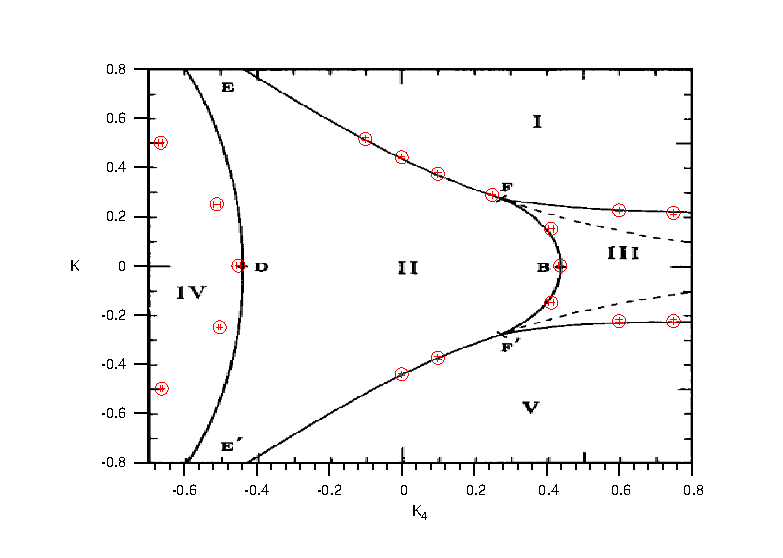
\includegraphics[scale=1]{graf/phases/new_phase_diag_back.eps}
	%~ \end{center}
	%~ \caption{Se presentan los puntos obtenidos en este trabajo para las transiciones de fase del modelo AT sobre el diagrama de fases publicado por Baxter\cite{baxter_book}.
	%~ En el caso de la transici\'on II$\rightarrow$IV, la curva es solo representativa, no se ha determiando su expresi\'on anal\'itica.}
	%~ \label{fig:phase_diag_back}
%~ \end{figure}

Los resultados hallados para todas las transiciones de fase estudiadas concuerdan con el diagrama de fases de la Fig. \ref{fig:AT_ph_diag_Baxter},
 y pueden verse superpuestos a este en la Fig. \ref{fig:phase_diag_back}, los c\'irculos rojos corresponden a los resultados n\'umericos obtenidos
 en este trabajo.\\
\newpage
